\section{Experimental Evaluation}
\paragraph{Dataset} Our proposed models are evaluated on the PASCAL VOC 2012 segmentation benchmark \citep{everingham2014pascal}, consisting of 20 foreground object classes and one background class. The original dataset contains $1,464$, $1,449$, and $1,456$ images for training, validation, and test, respectively. We use the extra annotations provided by \citet{hariharan2011semantic}, resulting in $10,582$ training images. The performance is measured in terms of pixel intersection-over-union (IOU) averaged across the 21 classes. 

\paragraph{Training} Our proposed models are built on top of the ``DeepLab'' and ``DeepLab-CRF'' models proposed by \citep{chen2014semantic}, which is composed of two main components: DCNN and Dense Conditional Random Field (DenseCRF) \citep{krahenbuhl2011efficient}. Similarly, we adopt piecewise training, decoupling the DCNN and CRF training stages, assuming the unary terms provided by the DCNN are fixed during CRF training. 

For DCNN training we employ the VGG-16 netwok which has been pre-trained on ImageNet. We fine-tuned the VGG-16 network on the VOC 21-way classification task by stochastic gradient descent on the cross-entropy loss function. We use a mini-batch of 20 images and initial learning rate of $0.001$ ($0.01$ for the final classifier layer), multiplying the learning rate by 0.1 at every 3000 iterations. We use momentum of $0.9$ and a weight decay of $0.0005$.

After the DCNN has been fine-tuned, we cross-validate the parameters of the Dense CRF model. The cross-validation is performed on a small subset of the validation set (we use 100 images). We use 10 iterations for the efficient mean field inference algorithm \citep{krahenbuhl2011efficient}. 

\subsection{Evaluation on Validation set}
The evaluations of our proposed models are mainly conducted on the PASCAL official validation set. 

\paragraph{Pixel Annotations}
\paragraph{Image Annotatins}
\paragraph{Pixel+Image Annotations}
\paragraph{Bounding Box (Bbox) Annotations}

\subsection{Evaluation on Test set}
After setting the model choices on the validation set, we evaluate our variant models on the PASCAL VOC 2012 official test set.

\begin{table}
  \centering
  \caption{{\bf{Pixel Annotations.}} Performance of our proposed models on the PASCAL VOC 2012 'val' set. First column, and second column show the number of strongly labeled images from PASCAL and MSCOCO used during training. The performance is evaluated in terms of mean IOU (\%).}
  \begin{tabular}{| c | c | c | c |}
    \hline
    \# PASCAL & \# MSCOCO & DeepLab & DeepLab-CRF \\
    \hline
    10,582 &   0     & 59.85 & 63.93  \\
    \hline
    10,582 & 123,287 & 64.51 & 67.98 \\
    \hline
    \end{tabular}
  \label{tb:pixel_annot}
\end{table}

\begin{table}[t]
  \centering
  \caption{{\bf Pixel+Image Annotations.} }
  \scalebox{0.8}{
  %\addtolength{\tabcolsep}{-2.0pt}
  \begin{tabular}{|c|c|c|c|}
    \hline
    {\bf Weak} & {\bf Strong} & \multirow{2}{*}{DeepLab} & \multirow{2}{*}{DeepLab-CRF}\\
    \cline{1-2}
    \# PASCAL & \# PASCAL & & \\
    \hline
    10,582   &    0    & 20.25  & 20.77   \\
    \hline
    10,582   &    0    & 34.22* & 38.23*  \\
    \hline
    10,382   &  200    & 44.05  & 47.57   \\
    \hline
    10,082   &  500    & 52.52  & 56.89   \\
    \hline
    9,832    &  750    & 55.04  & 58.82   \\
    \hline
    9,582    &  1,000  & 56.79  & 60.48   \\
    \hline
    9,118    &  1,464  & {\bf 58.30}  & {\bf 61.90}   \\
    \hline
    5,000    &  1,464  & 57.02  & 60.48   \\
    \hline
      0      &  1,464  & 54.77  & 57.62   \\
    \hline
  \end{tabular}  
  }
  \label{tab:strong_weak_annot}
\end{table}

\begin{table}[t]
  \centering
  \caption{{\bf Pixel+Image Annotations with MSCOCO.} }
  \scalebox{0.77}{
  %\addtolength{\tabcolsep}{-2.0pt}
  \begin{tabular}{|c|c|c|c|c|}
    \hline
    {\bf Weak} & \multicolumn{2}{c|}{\bf Strong} & \multirow{2}{*}{DeepLab} & \multirow{2}{*}{DeepLab-CRF}\\
    \cline{1-3}
    \# MSCOCO & \# PASCAL & \# MSCOCO & & \\
    \hline
      0       & 10,582 & 0       & 59.85 & 63.93 \\
    \hline
      123,287 & 10,582 & 0       & 60.41 & 64.44 \\
    \hline
      0       & 10,582 & 5,000   & ?     &  ?    \\
    \hline
      118,287 & 10,582 & 5,000   & ?     &  ?    \\
    \hline    
      0       & 10,582 & 123,287 & 64.51 & 67.98 \\
    \hline
  \end{tabular}  
  }
  \label{tab:strong_weak_annot_coco}
\end{table}

\begin{table}
  \centering
  \caption{{\bf Segmentation estimation within bounding boxes.} Dense CRF is employed to estimate the ground-truth segmentation. Row 1 to Row 3: difficulty of the task in increasing order.} 
  \begin{tabular}{c c c c}
    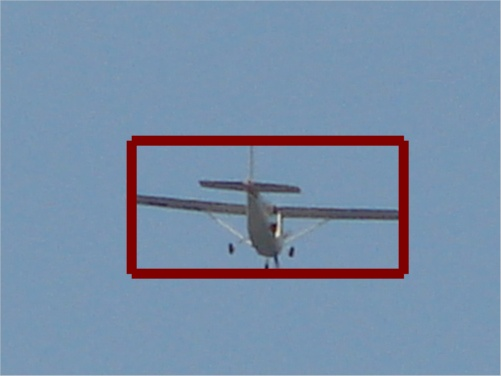
\includegraphics[width=0.21\linewidth]{fig/erode_bbox/img/2010_004063.jpg} & 
    
\includegraphics[width=0.21\linewidth]{fig/erode_bbox/gt/2010_004063.png} & 
    
\includegraphics[width=0.21\linewidth]{fig/erode_bbox/bbox/2010_004063.png} & 
    
\includegraphics[width=0.21\linewidth]{fig/erode_bbox/crf/2010_004063.png} \\    
    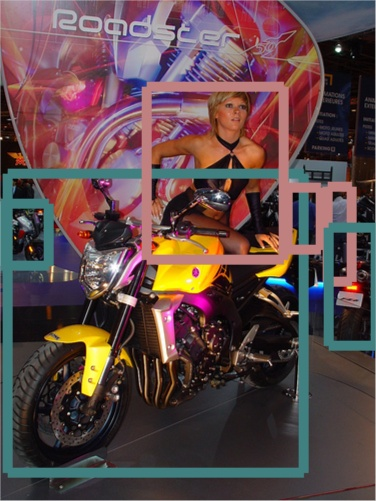
\includegraphics[width=0.21\linewidth]{fig/erode_bbox/img/2009_002382.jpg} & 
    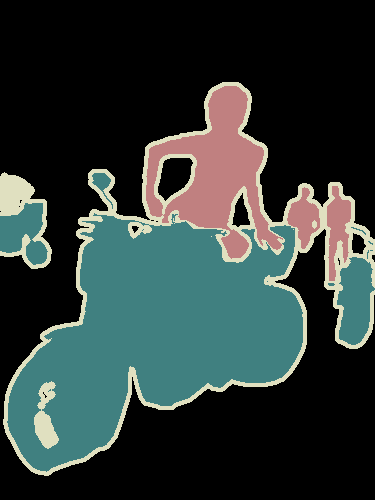
\includegraphics[width=0.21\linewidth]{fig/erode_bbox/gt/2009_002382.png} & 
    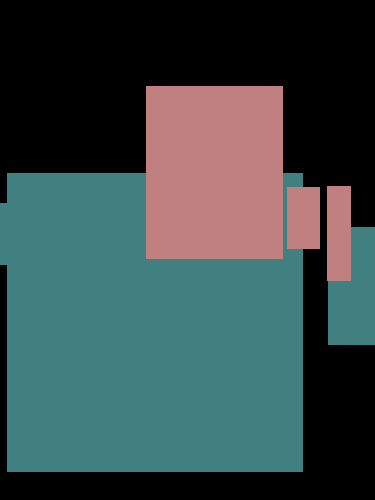
\includegraphics[width=0.21\linewidth]{fig/erode_bbox/bbox/2009_002382.png} & 
    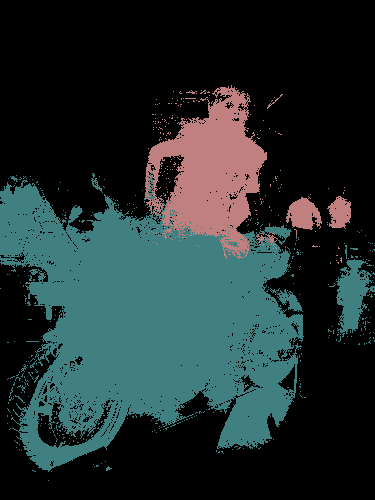
\includegraphics[width=0.21\linewidth]{fig/erode_bbox/crf/2009_002382.png} \\    
    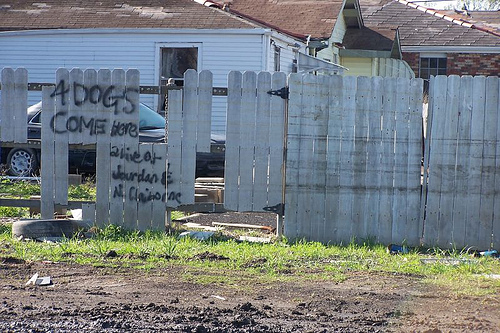
\includegraphics[width=0.21\linewidth]{fig/erode_bbox/img/2008_004339.jpg} & 
    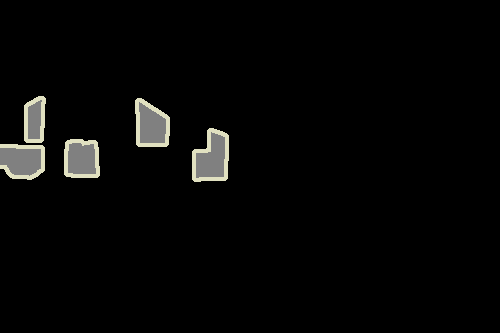
\includegraphics[width=0.21\linewidth]{fig/erode_bbox/gt/2008_004339.png} & 
    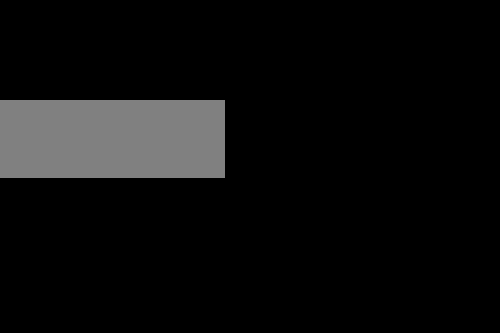
\includegraphics[width=0.21\linewidth]{fig/erode_bbox/bbox/2008_004339.png} & 
    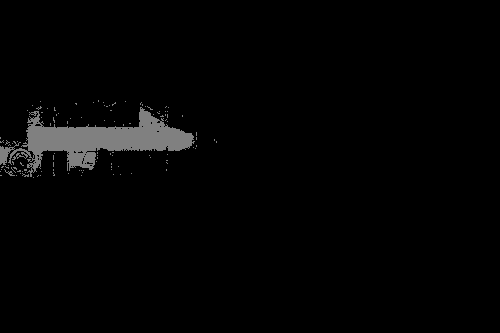
\includegraphics[width=0.21\linewidth]{fig/erode_bbox/crf/2008_004339.png} \\    
    Image & G.T. & Bbox & Est. G.T.
  \end{tabular}
\end{table}


\begin{table}
  \centering
  \caption{{\bf{Bounding Box Erosion Analysis.}}}
  \begin{tabular}{c | c}
    Bbox size & DenseCRF  \\
    \hline
    \hline
    80\%  & 65.59 \\
    60\%  & 68.80 \\
    40\%  & 71.57 \\
    20\%  & 72.23 \\
    \end{tabular}
  \label{tb:bbox_erosion}
\end{table}

\begin{table}
  \centering
  \caption{{\bf{Bounding Box Annotations.}}}
  \begin{tabular}{| c | c | c |}
    \hline
     & DeepLab & DeepLab-CRF \\
    \hline
    Naive method & 47.72 & 52.52 \\ 
    \hline
    DenseCRF     & 53.68 & 58.45 \\
    \hline
    \end{tabular}
  \label{tb:bbox_annot}
\end{table}


\begin{figure*}[!htbp]
  \centering
  %\vspace{-1.cm}
  \scalebox{0.82} {
  \begin{tabular}{c c c c c c}
    %\addtolength{\tabcolsep}{-6.5pt}
    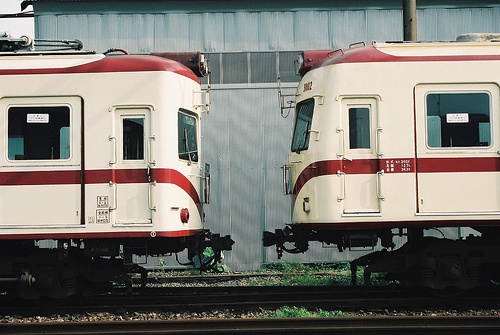
\includegraphics[height=0.11\linewidth]{fig/val_crf_vis/img/2007_000042.jpg} &
    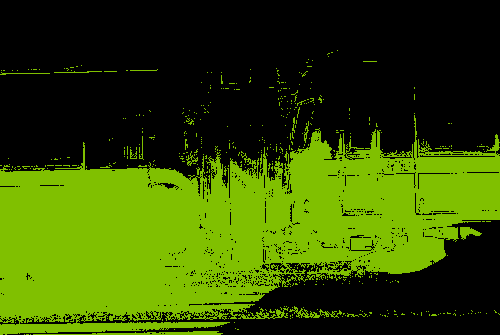
\includegraphics[height=0.11\linewidth]{fig/val_crf_vis/adaweak/2007_000042.png} &
    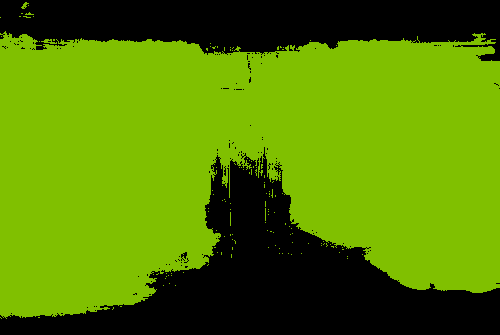
\includegraphics[height=0.11\linewidth]{fig/val_crf_vis/bbox/2007_000042.png} &
    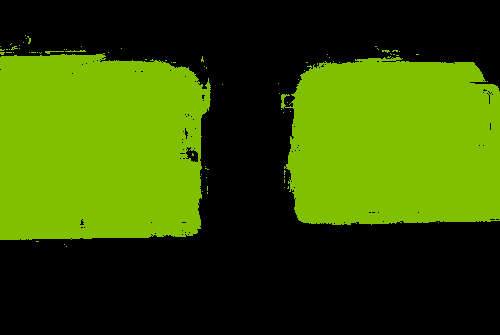
\includegraphics[height=0.11\linewidth]{fig/val_crf_vis/bbox_crf/2007_000042.png} &
    
\includegraphics[height=0.11\linewidth]{fig/val_crf_vis/strongweak/2007_000042.png} &
    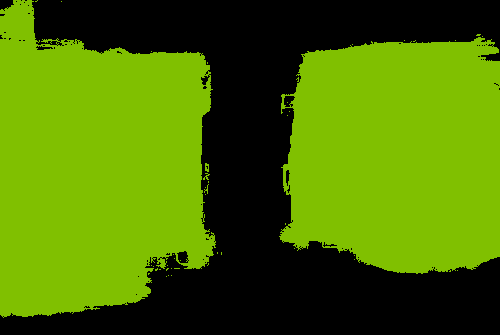
\includegraphics[height=0.11\linewidth]{fig/val_crf_vis/cocomix/2007_000042.png} \\
    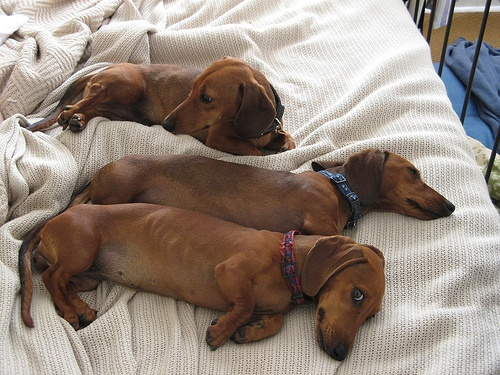
\includegraphics[height=0.122\linewidth]{fig/val_crf_vis/img/2007_002852.jpg} &
    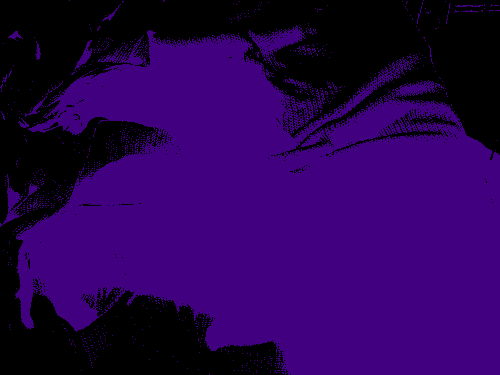
\includegraphics[height=0.122\linewidth]{fig/val_crf_vis/adaweak/2007_002852.png} &
    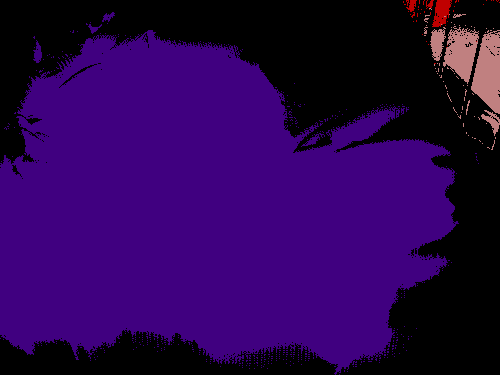
\includegraphics[height=0.122\linewidth]{fig/val_crf_vis/bbox/2007_002852.png} &
    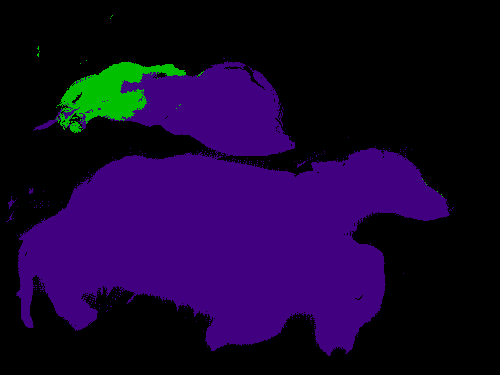
\includegraphics[height=0.122\linewidth]{fig/val_crf_vis/bbox_crf/2007_002852.png} &
    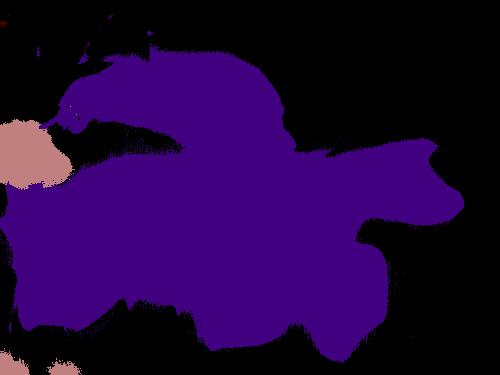
\includegraphics[height=0.122\linewidth]{fig/val_crf_vis/strongweak/2007_002852.png} &
    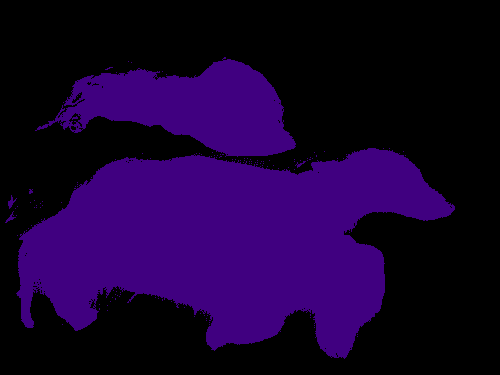
\includegraphics[height=0.122\linewidth]{fig/val_crf_vis/cocomix/2007_002852.png} \\
    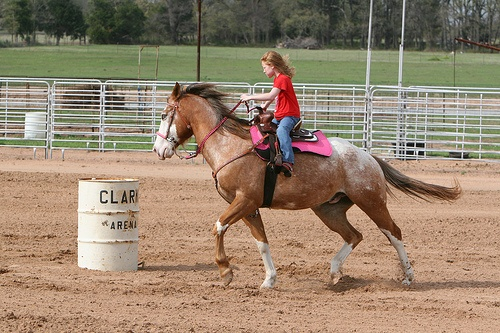
\includegraphics[height=0.11\linewidth]{fig/val_crf_vis/img/2007_003022.jpg} &
    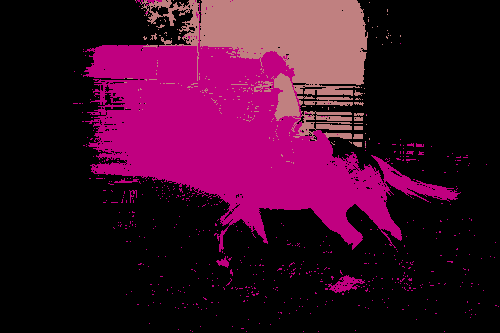
\includegraphics[height=0.11\linewidth]{fig/val_crf_vis/adaweak/2007_003022.png} &
    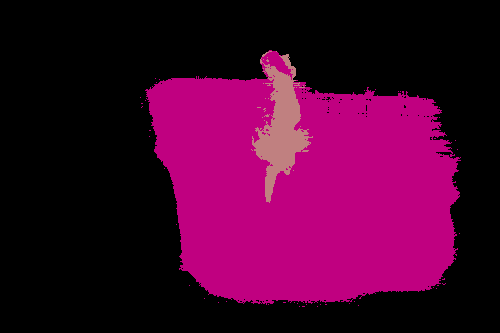
\includegraphics[height=0.11\linewidth]{fig/val_crf_vis/bbox/2007_003022.png} &
    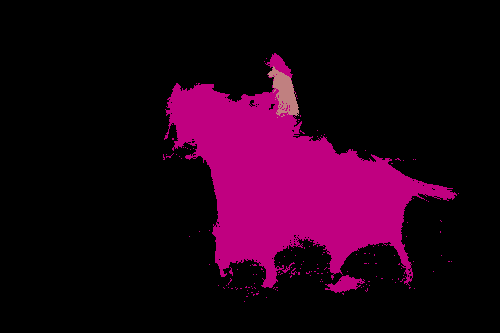
\includegraphics[height=0.11\linewidth]{fig/val_crf_vis/bbox_crf/2007_003022.png} &
    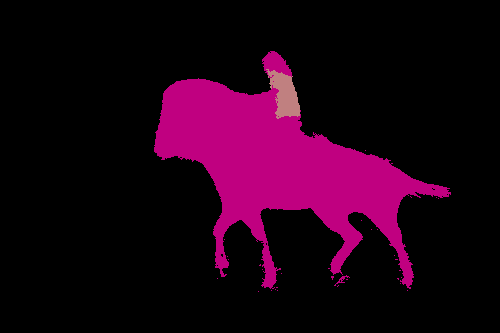
\includegraphics[height=0.11\linewidth]{fig/val_crf_vis/strongweak/2007_003022.png} &
    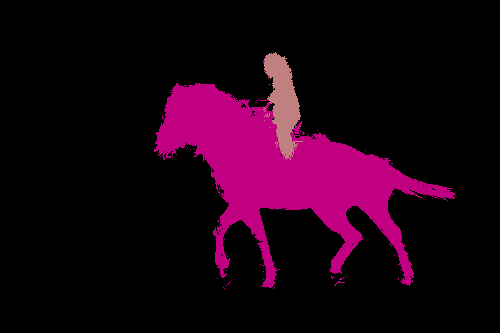
\includegraphics[height=0.11\linewidth]{fig/val_crf_vis/cocomix/2007_003022.png} \\
    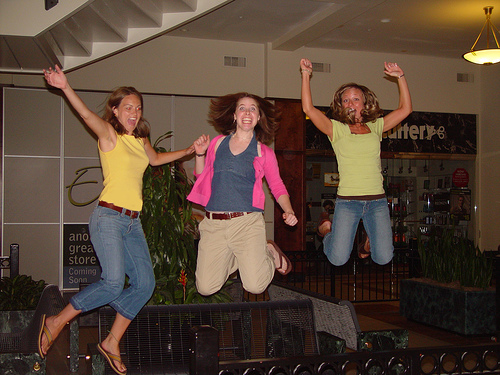
\includegraphics[height=0.123\linewidth]{fig/val_crf_vis/img/2008_003546.jpg} &
    
\includegraphics[height=0.123\linewidth]{fig/val_crf_vis/adaweak/2008_003546.png} &
    
\includegraphics[height=0.123\linewidth]{fig/val_crf_vis/bbox/2008_003546.png} &
    
\includegraphics[height=0.123\linewidth]{fig/val_crf_vis/bbox_crf/2008_003546.png} &
    
\includegraphics[height=0.123\linewidth]{fig/val_crf_vis/strongweak/2008_003546.png} &
    
\includegraphics[height=0.123\linewidth]{fig/val_crf_vis/cocomix/2008_003546.png} \\
    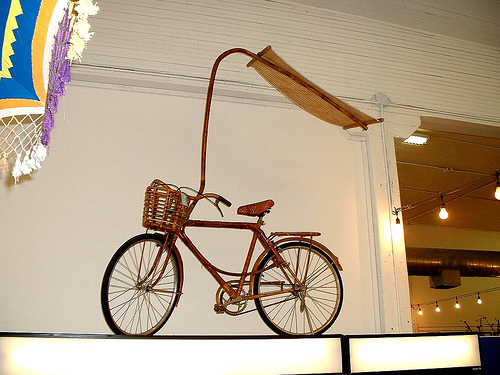
\includegraphics[height=0.123\linewidth]{fig/val_crf_vis/img/2008_004363.jpg} &
    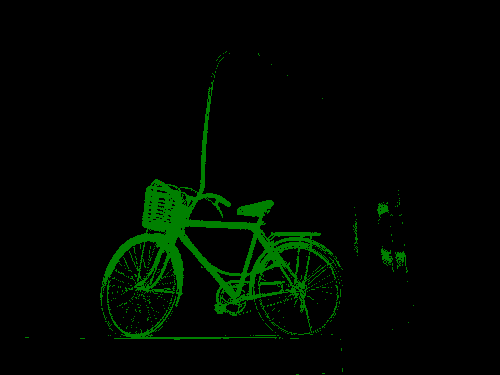
\includegraphics[height=0.123\linewidth]{fig/val_crf_vis/adaweak/2008_004363.png} &
    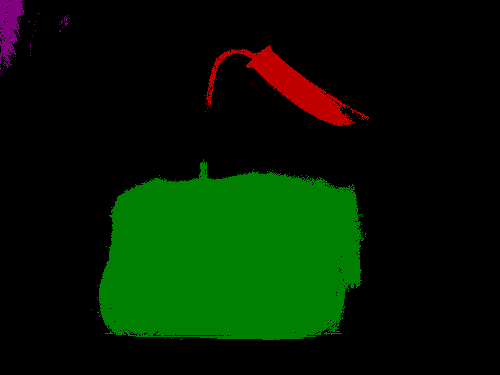
\includegraphics[height=0.123\linewidth]{fig/val_crf_vis/bbox/2008_004363.png} &
    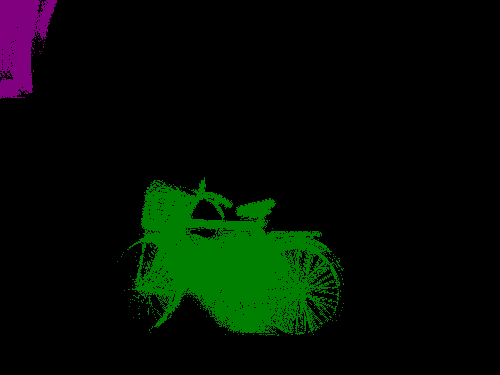
\includegraphics[height=0.123\linewidth]{fig/val_crf_vis/bbox_crf/2008_004363.png} &
    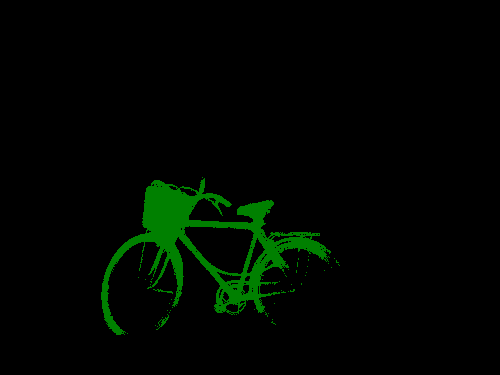
\includegraphics[height=0.123\linewidth]{fig/val_crf_vis/strongweak/2008_004363.png} &
    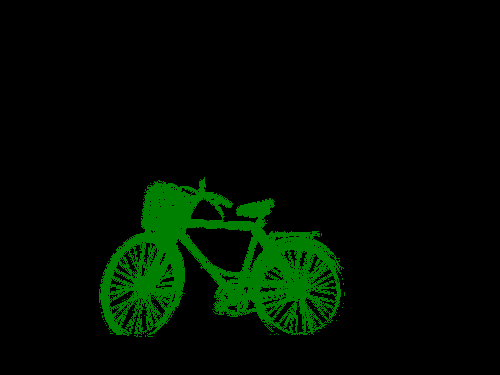
\includegraphics[height=0.123\linewidth]{fig/val_crf_vis/cocomix/2008_004363.png} \\
    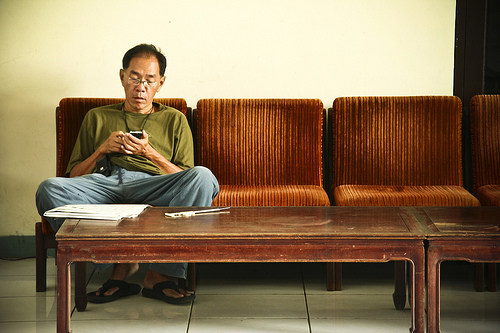
\includegraphics[height=0.11\linewidth]{fig/val_crf_vis/img/2009_001299.jpg} &
    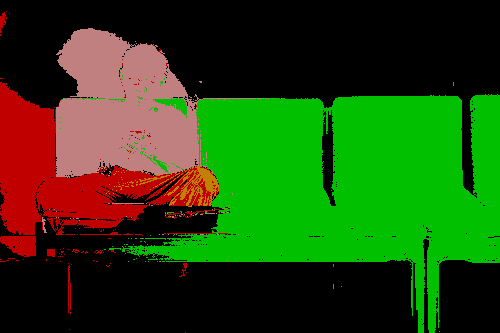
\includegraphics[height=0.11\linewidth]{fig/val_crf_vis/adaweak/2009_001299.png} &
    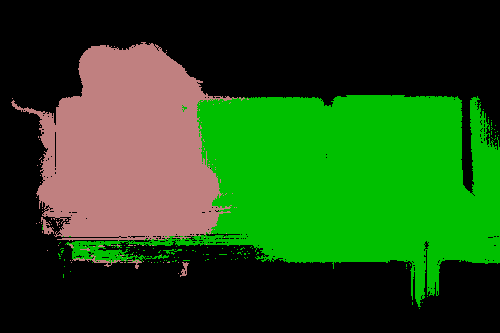
\includegraphics[height=0.11\linewidth]{fig/val_crf_vis/bbox/2009_001299.png} &
    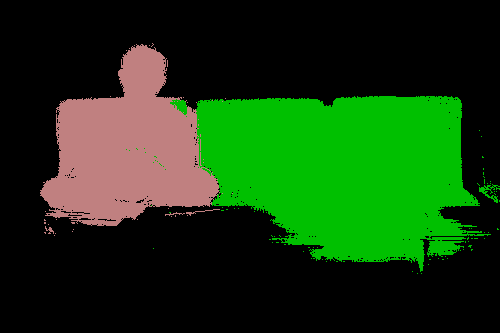
\includegraphics[height=0.11\linewidth]{fig/val_crf_vis/bbox_crf/2009_001299.png} &
    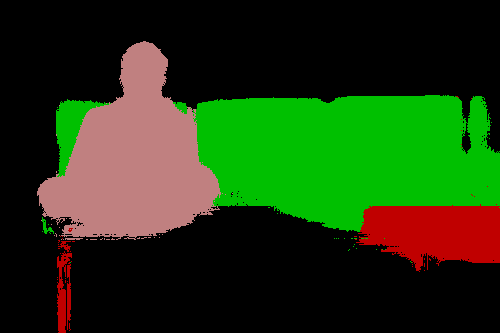
\includegraphics[height=0.11\linewidth]{fig/val_crf_vis/strongweak/2009_001299.png} &
    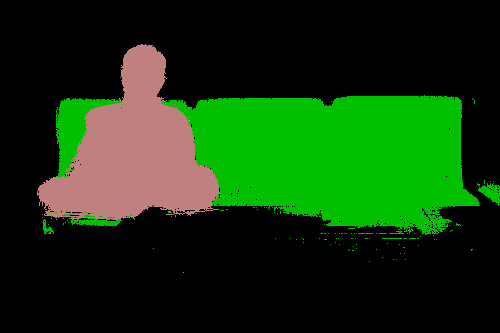
\includegraphics[height=0.11\linewidth]{fig/val_crf_vis/cocomix/2009_001299.png} \\
    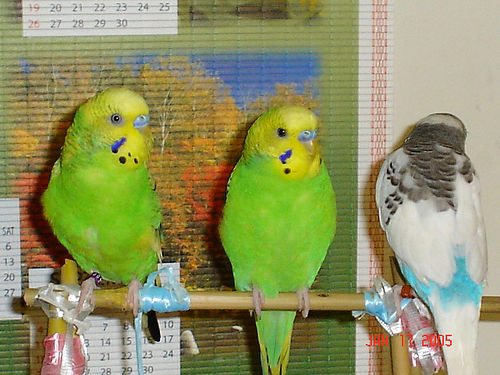
\includegraphics[height=0.123\linewidth]{fig/val_crf_vis/img/2010_004994.jpg} &
    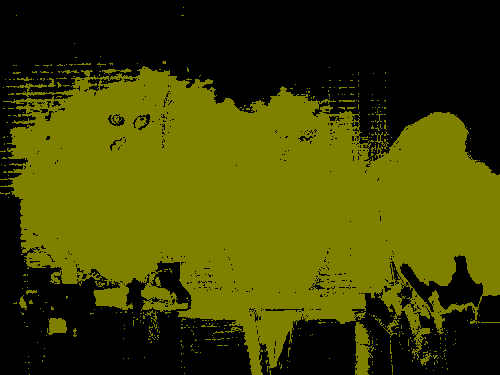
\includegraphics[height=0.123\linewidth]{fig/val_crf_vis/adaweak/2010_004994.png} &
    \includegraphics[height=0.123\linewidth]{fig/val_crf_vis/bbox/2010_004994.png} &
    \includegraphics[height=0.123\linewidth]{fig/val_crf_vis/bbox_crf/2010_004994.png} &
    \includegraphics[height=0.123\linewidth]{fig/val_crf_vis/strongweak/2010_004994.png} &
    \includegraphics[height=0.123\linewidth]{fig/val_crf_vis/cocomix/2010_004994.png} \\
    \includegraphics[height=0.122\linewidth]{fig/val_crf_vis/img/2011_002322.jpg} &
    \includegraphics[height=0.122\linewidth]{fig/val_crf_vis/adaweak/2011_002322.png} &
    \includegraphics[height=0.122\linewidth]{fig/val_crf_vis/bbox/2011_002322.png} &
    \includegraphics[height=0.122\linewidth]{fig/val_crf_vis/bbox_crf/2011_002322.png} &
    \includegraphics[height=0.122\linewidth]{fig/val_crf_vis/strongweak/2011_002322.png} &
    \includegraphics[height=0.122\linewidth]{fig/val_crf_vis/cocomix/2011_002322.png} \\
    \includegraphics[height=0.13\linewidth]{fig/val_crf_vis/img/2007_001630.jpg} &
    \includegraphics[height=0.13\linewidth]{fig/val_crf_vis/adaweak/2007_001630.png} &
    \includegraphics[height=0.13\linewidth]{fig/val_crf_vis/bbox/2007_001630.png} &
    \includegraphics[height=0.13\linewidth]{fig/val_crf_vis/bbox_crf/2007_001630.png} &
    \includegraphics[height=0.13\linewidth]{fig/val_crf_vis/strongweak/2007_001630.png} &
    \includegraphics[height=0.13\linewidth]{fig/val_crf_vis/cocomix/2007_001630.png} \\
    \includegraphics[height=0.15\linewidth]{fig/val_crf_vis/img/2007_005331.jpg} &
    \includegraphics[height=0.15\linewidth]{fig/val_crf_vis/adaweak/2007_005331.png} &
    \includegraphics[height=0.15\linewidth]{fig/val_crf_vis/bbox/2007_005331.png} &
    \includegraphics[height=0.15\linewidth]{fig/val_crf_vis/bbox_crf/2007_005331.png} &
    \includegraphics[height=0.15\linewidth]{fig/val_crf_vis/strongweak/2007_005331.png} &
    \includegraphics[height=0.15\linewidth]{fig/val_crf_vis/cocomix/2007_005331.png} \\
\hline \hline
    \includegraphics[height=0.11\linewidth]{fig/val_crf_vis/img/2007_000830.jpg} &
    \includegraphics[height=0.11\linewidth]{fig/val_crf_vis/adaweak/2007_000830.png} &
    \includegraphics[height=0.11\linewidth]{fig/val_crf_vis/bbox/2007_000830.png} &
    \includegraphics[height=0.11\linewidth]{fig/val_crf_vis/bbox_crf/2007_000830.png} &
    \includegraphics[height=0.11\linewidth]{fig/val_crf_vis/strongweak/2007_000830.png} &
    \includegraphics[height=0.11\linewidth]{fig/val_crf_vis/cocomix/2007_000830.png} \\
    \includegraphics[height=0.11\linewidth]{fig/val_crf_vis/img/2007_001175.jpg} &
    \includegraphics[height=0.11\linewidth]{fig/val_crf_vis/adaweak/2007_001175.png} &
    \includegraphics[height=0.11\linewidth]{fig/val_crf_vis/bbox/2007_001175.png} &
    \includegraphics[height=0.11\linewidth]{fig/val_crf_vis/bbox_crf/2007_001175.png} &
    \includegraphics[height=0.11\linewidth]{fig/val_crf_vis/strongweak/2007_001175.png} &
    \includegraphics[height=0.11\linewidth]{fig/val_crf_vis/cocomix/2007_001175.png} \\
    Image & adaweak & bbox & bbox-crf & strongweak & cocomix \\
  \end{tabular}
  }
  %\vspace{-0.3cm}
  \caption{Visualization results on VOC 2012-val. For each row, we show the input image, the segmentation result delivered by adaweak, bbox, bbox-crf, strongweak, coco. The results are refined by DenseCRF. We show difficult examples in the last two rows.} 
  \label{fig:ValResults}
\end{figure*}





{\color{blue} REMEMBER to put the links (test results) in the supplementary material if main paper has no space.}
\begin{table*}[ht]\scriptsize
 \caption{Labeling IoU (\%) on the PASCAL VOC 2012 test set, using the trainval set for training.}
\setlength{\tabcolsep}{3pt}
%\hspace{-1.8cm}
\resizebox{2\columnwidth}{!}{
\begin{tabular}{|c||c*{20}{|c}||c|}
\hline 
Method          & bkg &  aero & bike & bird & boat & bottle& bus & car  &  cat & chair& cow  &table & dog  & horse & mbike& person& plant&sheep& sofa &train & tv   & mean \\
\hline \hline
Weak-sppxl      & 74.7 & 38.8 & 19.8 & 27.5 & 21.7 & 32.8 & 40.0 & 50.1 & 47.1 & 7.2 & 44.8 & 15.8 & 49.4 & 47.3 & 36.6 & 36.4 & 24.3 & 44.5 & 21.0 & 31.5 & 41.3 & 35.8 \\
Weak-seg        & 78.7 & 48.0 & 21.2 & 31.1 & 28.4 & 35.1 & 51.4 & 55.5 & 52.8 & 7.8 & 56.2 & 19.9 & 53.8 & 50.3 & 40.0 & 38.6 & 27.8 & 51.8 & 24.7 & 33.3 & 46.3 & 40.6 \\
\hline \hline
Hypercolumn-SDS & 88.9 & 68.4 & 27.2 & 68.2 & 47.6 & 61.7 & 76.9 & 72.1 & 71.1 & 24.3 & 59.3 & 44.8 & 62.7 & 59.4 & 73.5 & 70.6 & 52.1 & 63.0 & 38.1 & 60.0 & 54.1 & 59.2 \\   
MSRA-CFM        & -    & 75.7 & 26.7 & 69.5 & 48.8 & 65.6 & 81.0 & 69.2 & 73.3 & 30.0 & 68.7 & 51.5 & 69.1 & 68.1 & 71.7 & 67.5 & 50.4 & 66.5 & 44.4 & 58.9 & 53.5 & 61.8 \\
FCN-8S          & -    & 76.8 & 34.2 & 68.9 & 49.4 & 60.3 & 75.3 & 74.7 & 77.6 & 21.4 & 62.5 & 46.8 & 71.8 & 63.9 & 76.5 & 73.9 & 45.2 & 72.4 & 37.4 & 70.9 & 55.1 & 62.2 \\
TTI-Zoomout-16  & 89.8 & 81.9 & 35.1 & 78.2 & 57.4 & 56.5 & 80.5 & 74.0 & 79.8 & 22.4 & 69.6 & 53.7 & 74.0 & 76.0 & 76.6 & 68.8 & 44.3 & 70.2 & 40.2 & 68.9 & 55.3 & 64.4 \\
DeepLab-CRF     & 92.1 & 78.4 & 33.1 & 78.2 & 55.6 & 65.3 & 81.3 & 75.5 & 78.6 & 25.3 & 69.2 & 52.7 & 75.2 & 69.0 & 79.1 & 77.6 & 54.7 & 78.3 & 45.1 & 73.3 & 56.2 & 66.4 \\ 
\hline \hline
adaweak & 76.4 & 37.0 & 17.6 & 38.2 & 26.6 & 37.1 & 51.9 & 43.3 & 48.1 & 16.8 & 44.6 & 27.9 & 46.5 & 46.2 & 46.6 & 30.3 & 28.9 & 42.0 & 30.0 & 43.8 & 39.3 & 39.0 \\
bbox    & 82.9 & 43.6 & 22.5 & 50.5 & 45.0 & 62.5 & 76.0 & 66.5 & 61.2 & 25.3 & 55.8 & 52.1 & 56.6 & 48.1 & 60.1 & 58.2 & 49.5 & 58.3 & 40.7 & 62.3 & 61.1 & 54.2 \\
bbox-crf & 89.9 & 69.3 & 28.2 & 71.9 & 43.4 & 59.7 & 74.3 & 69.0 & 76.7 & 23.5 & 64.6 & 47.1 & 71.0 & 64.0 & 72.8 & 72.4 & 50.4 & 72.0 & 40.2 & 63.4 & 44.5 & 60.4 \\
strong-weak(1.5K) & 91.4 & 77.3 & 38.2 & 73.9 & 47.6 & 57.9 & 80.0 & 76.4 & 74.7 & 22.8 & 70.0 & 42.0 & 70.9 & 71.9 & 79.1 & 70.7 & 47.8 & 77.1 & 36.1 & 68.1 & 59.8 & 63.5 \\
strong-weak(3K) & 92.3 & 81.3 & 43.8 & 78.3 & 50.2 & 60.4 & 81.2 & 77.5 & 77.5 & 26.8 & 70.8 & 47.0 & 74.8 & 73.0 & 80.8 & 76.0 & 50.8 & 78.0 & 39.7 & 72.9 & 60.9 & 66.4 \\
DeepLabe-CRF-COCO & 93.2 & 85.3 & 36.2 & 84.8 & 61.2 & 67.5 & 84.7 & 81.4 & 81.0 & 30.8 & 73.8 & 53.8 & 77.5 & 76.5 & 82.3 & 81.6 & 56.3 & 78.9 & 52.3 & 76.6 & 63.3 & 70.4 \\
\hline
 \end{tabular}
} \label{tab:voc2012}
\end{table*}
